\documentclass{frontiersSCNS}
\usepackage{url,lineno}
\linenumbers
\copyrightyear{}
\pubyear{}

\def\journal{Human Neuroscience}
\def\DOI{}
\def\articleType{Research Article}
\def\keyFont{\fontsize{8}{11}\helveticabold }

\def\firstAuthorLast{Brooks, Cid de Garcia, and Marantz}

\def\Authors{Teon Brooks\,$^{1,*}$, Daniela Cid de Garcia\,$^{2,*}$ and Alec Marantz\,$^{1,3,4}$}

\def\Address{$^{1}$New York University, Department of Psychology, New York, NY, USA\\
$^{2}$Universidade Federal do Rio de Janeiro, Department of Anglo-Germanic Languages, Rio de Janiero, RJ, BR\\
$^{3}$New York University, Department of Linguistics, New York, NY, USA \\
$^{4}$NYUAD Institute, New York University Abu Dhabi, Abu Dhabi, UAE}

\def\corrAuthor{Teon Brooks}
\def\corrAddress{Department of Psychology, New York University, 6 Washington Place, 2nd Floor, New York , NY, USA}
\def\corrEmail{teon@nyu.edu}

\extraAuth{Daniela Cid de Garcia\\Department of Anglo-Germanic Languages, Federal University of Rio de Janeiro, Av. Horácio Macedo, 2151, Sala D204, CEP 21941-917, Cidade Universitária, Rio de Janeiro - RJ, BR, cid.daniela@gmail.com}


\begin{document}
\onecolumn
\firstpage{1}

\title[Integrating morpheme form and meaning]{Evidence for Morphological Recomposition in Compound Words using MEG}
\author[\firstAuthorLast ]{\Authors}
\address{}
\correspondance{}

\topic{Morphologically complex words in the mind/brain}
\maketitle

\begin{abstract}

Psycholinguistic and M/EEG studies of lexical processing show convergent evidence for a morpheme-based route that involves early decomposition into constituent morphemes and post-lexical combinatorial semantic operations.  Considering that both semantically transparent (e.g. sailboat) and semantically opaque (e.g. bootleg) compounds undergo decomposition at the earlier stages of lexical processing, subsequent combinatorial operations should account for the difference in the meaning retrieval of these different word types.  In this study we use magnetoencephalography (MEG) to pinpoint the neural bases of this combinatorial stages in English compound word recognition and production. MEG data were acquired while participants performed a word naming task in which four word types (transparent, opaque, novel and simplex) were contrasted in two priming conditions (repetition and constituent). We found two regions of interest implicated in morphological recomposition, the Left Anterior Temporal Lobe (LATL), and the posterior Superior Temporal Gyrus (pSTG).  Previous studies using sentences and phrases have highlighted the LATL as implicated with basic combinatorial operations, and the posterior temporal lobe for lexical access. Results are in tune with decomposition models and suggest the existence of a word processing dynamics that is modulated by morphological complexity and semantic transparency in spatially distinct brain areas.

\tiny
 \keyFont{ \section{Keywords:} complex words, compounds, MEG, LATL, pSTG, lexical access, word naming, semantic transparency } 
%All article types: you may provide up to 8 keywords; at least 5 are mandatory.
\end{abstract}

\section{Introduction}

	Some words are simple and some words are not. This, at first, sounds like a very trivial tautology, but the investigation over whether complex words – words that have more than one morpheme – are simply stored in whole word form \citep*{Butterworth:1983, Giraudo:2001} or in morphemic parts has been entertaining, provocative, and contentious in the field of lexical processing for the last forty years of research \citep*{Rastle:2003}. A comprehensive description of how words are both stored and retrieved requires the understanding of how form and meaning are connected, and how this connection unfolds in time in natural speech. On the one hand, understanding the mechanisms involved in the comprehension of linguistic expression involves examining how perceptual information is analyzed from the moment in which the visual or auditory input is presented until the activation of the intended meaning happens. On the other hand, a model of language processing willing to describe the production of language expressions should account for how the intended message is conceived, planned, and executed to convey the intended meaning. A well-described model of lexical processing must first characterize the unit of measurement. This study focuses on elucidating the units of processing in word retrieval and the planning units in production.

	This idea of simplicity and complexity in word storage was first discussed in the classic affix-stripping model \citep*{Taft:1975} where in lexical decision, we saw effects on reaction times such that pseudo-complex words with plausible stems took longer to make a lexical decision and were often selected as incorrectly, while words without this complex structure did not exhibit this slow down effect. This was very early evidence that structure within a word matters, in particular to reach lexical access. The evidence has mounted both in favor \citep*{Taft:2004, Marslen-Wilson:1994, Rastle:2004} and disapproval \citep*{Butterworth:1983, Giraudo:2001}, but the evidence against morphological sensitivity in lexical access has diminished giving rise to processing models where morphology is a necessary stage in processing. These psychological models make a variety of prediction to the stages and time-course of lexical access, but there is a lack of evidence for their realization in the brain. This study seeks to explain how and where the integration of morpheme meaning occurs.

	One way to look at lexical processing is to see if activating morphological structure can modulate the accessibility within a complex word. Cross-modal studies \citep{Marslen-Wilson:1994} showed that priming in lexical decisions only occurred when the prime and target had related meanings (e.g., departure primed depart but department did not) while other studies \citep*{Zwitserlood:1994} found that priming did not depend on a semantic relationship between the prime and target. However, masked priming studies that manipulate semantic transparency find facilitation effects regardless of whether prime and target share the same morphological root \citep*{Rastle:2004, Longtin:2003, Fiorentino:2007, McCormick:2008}.  Facilitation effects are found for every complex word that can be segmented in existing morphemes, which means that pairs like \textit{corn-corner} and \textit{boot-bootleg} obtain facilitation as much as pairs like \textit{clean-cleaner} and \textit{tea-teacup}, even though there is no morphological relationship in the former pairs.

	These results have gained support in electrophysiology with MEG studies showing activation peaking around 170 ms after the presentation of a stimulus (M170 on morphological decomposition: \citealt{Solomyak:2010}) and a somewhat later in EEG, at around 250ms (N250: \citealt{Morris:2007}). Their source generator has been localized to the left fusiform gyrus \citep*{Dehaene:2010, Solomyak:2010}.
If decomposition is true for every word that can be superficially segmented in whatever looks like existing morphemes, regardless of whether the word is indeed morphologically complex or not, research on visual word recognition should shift the focus now to the subsequent mechanisms engaged to activate the actual meaning of the target word.  \citet*{Meunier:2007} suggest that word activation comes to play at stages, which include at least one early stage for morphological decomposition and a later stage for semantic integration. \citet*{Fiorentino:2013} presents evidence for a morpheme-based route for word activation that includes decomposition into morphological constituents and combinatorial processes operating on these representations.  Since previous studies have shown that early decomposition triggered by morphological structure happens instinctively for transparent and opaque words, the difference between these two word types may take place during the stage of combinatorial operations.

	Another way to look at lexical processing of complex words is to look at lexical access. It follows from decomposition models that morpheme units should undergo some lexical access in order for their meanings to be recombined. In a review by \citet*{Hickok:2007}, their dual stream model for speech processing proposed a lexical interface located in the posterior middle temporal gyrus (pMTG), which is responsible for linking the phonological and semantic information, and more broadly the posterior lateral temporal lobe for its involvement in lexical semantics. \citet*{Lau:2008} also suggested a more posterior region of the temporal lobe as an ideal candidate for lexical storage highlighting the posterior middle temporal gyrus as well as its neighboring posterior superior and inferior lobules in their involvement in lexical representation.

	A final way to look at lexical processing is to look at composition. There are proposals for a general binding mechanism for basic composition proposed by \citet*{Bemis:2011} that may play a role at the word-level. In a minimum composition paradigm, \citep{Bemis:2011} found that two composable items, an adjective-noun phrase, revealed more activation in the LATL than two non-composable items, a random letter string and word. This was taken as evidence of the most basic of combinatorial processing. This region would thus be responsible for combinatorial operations with morphemes. Semantic transparency, the degree to which morpheme meaning correspond to the overall word meaning, can be used to test whether this region is engaged when determining the semantic fit within a complex word. In this experiment, we will use compound to vary semantic transparency since they consist of existing free morphemes with different levels of semantic interactions. Thus, semantically opaque compounds (e.g. bootleg) that have no relationship between its parts and its meaning would fail tests of semantic fit while semantically transparent compounds (e.g. butterfly) would pass resulting in differential processing in this region. Since compounds are formed by independent morphemes, this provides an interesting basis to studying effects of intralexical semantic composition as an analogue to the ones studied at the phrase level.

	Thus, a model of complex word recognition would require at least these three stages of process: parsing into basic units (decomposition), access of their meanings (lexical access) and the recomposition of these word forms with their meaning. We propose using a partial-repetition priming paradigm, similar to the ones used in masked priming studies, with a word naming production task to uncover the stages involved in lexical processing. This task will be done while brain activity is recorded using MEG. This study contributes to the work of characterizing the neural bases of lexical processing of complex words by providing evidence for these proposed stages of processing, looking at compound words, while linking them to their neural correlates.

\section{Material \& Methods}

\textit{Participants.} Eighteen right-handed native speakers of English, with normal or corrected vision, participated in this experiment. Two were excluded due to large number of trial rejections (>25 \%). Details for rejection are described in the procedure.

\textit{Material.}  All stimuli consisted of English bi-morphemic compound (e.g. teacup) and morphologically simplex (e.g. spinach) nouns, matched for length and surface frequency. We manipulated semantic transparency, including fully semantically transparent (e.g. teacup) words, in which both constituent morphemes have a semantic relationship to the meaning of the whole compound, and fully semantically opaque words (e.g. hogwash), in which neither of the constituent morphemes have a semantic relationship to the compound meaning.

	Three hundred eleven English compounds were compiled from previous studies \citep*{Drieghe:2010, Fiorentino:2007, Fiorentino:2009, Juhasz:2003} and categorized in terms of semantic transparency by means of a semantic relatedness task conducted using the Amazon Mechanical Turk tool. In this task, 20 participants were asked to judge, on a 1-7 scale, how much each constituent of the compounds related to the whole word.  On the scale, 1 corresponded to “unrelated” and 7 corresponded to “very related”.  Each participant was randomly presented to one of the constituents of each compound.  Compounds were classified as semantically opaque (henceforth opaque) if the sum of the scores of their constituents were within the interval 2-6, and as semantically transparent (henceforth transparent) if the sum were within the interval 10-14. For example, the opaque compound \textit{deadline} received a summed rating of 3.76 with \textit{dead} contributing a transparency rating of 1.44 and \textit{line} contributing a rating of 2.32. Similarly, the compound \textit{dollhouse} received a summed rating of 11.79 with \textit{doll} contributing a transparency rating of 6.47 and \textit{house} contributing a rating of 5.32. Sixty compounds were selected for each word type. This method of semantic transparency norming and the ratings were consistent with the mentioned prior studies. The orthographic simple words were pooled from \citet{Rastle:2004} and the English Lexicon Project \citep*{Balota:2007}.	
	
	We also included novel English compounds (henceforth novel, e.g. ladyfork) to explore compositionality in novel words.  Since these words are not represented in the mental lexicon of the participants  \citep{Libben:1998}, obligatory combinatorial effects should be found during word recognition. These words were generated using the remaining words from the relational task, that is, the words that were not selected for the Transparent and Opaque categories.  The constituents of these compounds were randomly recombined to form novel English compounds.  In order to avoid the accidental creation of an existing word, the frequencies of these novel words were checked in the English Lexicon Project \citep{Balota:2007} so that the selected words had a surface frequency of zero. The orthographic simplex words (henceforth ortho: e.g. spinach) were selected to have an embedded word within it but with no morphological relationship. Also, it was constrained and selected such that if the embedded word were removed, the remaining word part would have no meaning.
 
\textit{Design.}  The four different word types were contrasted in two priming conditions: full repetition and partial (constituent) repetition (See Figure \ref{tab:Design-Matrix}).  For the repetition priming condition, the same compound was used as prime and target (e.g. TEACUP-teacup). For the constituent priming, we used the first constituent of the compound as the prime (e.g. TEA-teacup). For the orthos, the embedded word was used as the constituent in the constituent priming condition (e.g. SPIN-spinach). These two priming conditions were paired to control conditions in which the prime had no semantic relationship to the target (e.g. DOORBELL-teacup; DOOR-teacup). 

\begin{table}
\begin{tabular}{|c||c|c||c|c||c|c||c|c|}
\hline 
\multicolumn{1}{|c||}{\multirow{}{}{}} & \multicolumn{2}{c||}{Transparent} & \multicolumn{2}{c||}{Opaque} & \multicolumn{2}{c||}{Novel} & \multicolumn{2}{c|}{Ortho}\tabularnewline
\cline{2-9} 
 & prime & target & prime & target & prime & target & prime & target\tabularnewline
\hline 
\hline 
control & doorbell & teacup & heirloom & hogwash & keybook & ladyfork & brothel & spinach\tabularnewline
\hline 
identity & teacup & teacup & hogwash & hogwash & ladyfork & ladyfork & spinach & spinach\tabularnewline
\hline 
\hline 
control & door & teacup & heir & hogwash & key & ladyfork & broth & spinach\tabularnewline
\hline 
constituent & tea & teacup & hog & hogwash & lady & ladyfork & spin & spinach\tabularnewline
\hline 
\end{tabular}\caption{\label{tab:Design-Matrix} Design Matrix}
\end{table}

\textit{Procedure.} All participants read all the items in all conditions (960 total), which were divided in four lists of 240 words and randomized within each list.  The order of presentation of the lists was counterbalanced between subjects.  The experimental task was word naming: subjects were presented with word pairs, and they were asked to read out loud the second word of each pair.  This task allowed for the use of every presented item to be included in the analysis. Each trial began with the presentation of a fixation cross, followed by the prime, then the target. Each of these visual presentations was presented for 300 ms with an inter-stimulus interval of 600ms. We recorded the onset latency to speech and the utterance from each subject for behavioral analysis.

Before the experiment, the head shape of each participant was digitalized using the Polhemus Fastscan system, along with five head position indicator points, which are used to co-register the head position with respect to the MEG during acquisition.  The head shape is used during the analysis to co-register the head to participants’ MRIs. For half of the participants, MRIs were not provided, therefore we scaled the common reference brain that is provided in FreeSurfer to make the size of these participants’ head.

	During the experiment, participants remain lying in a magnetically shielded room as the brain activity is monitored from the MEG. The experiment was projected onto a translucent screen so the participant could read and perform the task. The MEG data was collected using a axial whole-head gradiometer system with 157 channels and three reference channels (Kanazawa Institute of Technology, Nonoichi, Japan).  The recording was conducted in direct current (DC), that is, without high-pass filter, and with 300 Hz low-pass filter and 60 Hz notch filter.

\textit{Analysis.} We examined onset latency, the reaction time to speak, to evaluate the effects of morphological structure based on \citep{Fiorentino:2007}, which predicts that since reaction time is sensitive to lexical processes, compounds will differ from single words, due to the properties of the constituents rather than the whole word, whereas a non-decompositional account predicts no differences due to word structure. Thus, onset latency can be used to disentangle whether or not there is a decomposition effect. The behavioral data were analyzed using traditional analysis of variance.

After brain data acquisition, we applied a Continuously Adjusted Least-Squares Method \citep{Adachi:2001}, a noise reduction procedure in the MEG160 software (Yokogawa Electric Corporation and Eagle Technology Corporation, Tokyo, Japan), and a bandpass filter of 1-40 Hz.  The recording of the whole experiment was segmented in epochs of interest, from -100 ms before to 600 ms after stimulus onset.  We rejected trials in which the maximal peak-to-peak amplitude exceeded the limit of 4000fT. Sensor channels were marked as bad and discarded for each subject if the channel’s peak-to-peak rejection exceeded 10%. 

A noise-covariance matrix was computed using a time epoch from -200 ms to the onset of the fixation cross.  For participants with MRIs, cortical reconstructions were generated using FreeSurfer resulting in a source space of 5124 vertices (CorTechs Labs Inc., La Jolla, CA and MGH/HMS/MIT Athinoula A. Martinos Center for Biomedical Imaging, Charleston, MA). For participants without MRIs, the headshape-constrained FreeSurfer average brain was used. A boundary-element model (BEM) method was used to model activity at each vertex to calculate a forward solution. An inverse solution was generated using this forward model and noise-covariance matrix, and was computed with a fixed-orientation constraint. 
The sensor data for each subject was then projected into their individual source space using a cortically-constrained minimum norm estimate (all analyses were conducted using MNE-Python \citet*{Gramfort:2013, Gramfort:2013a}) resulting in noise-normalized dynamic statistical parameter maps (dSPMs). Subjects with more than 25\% of the trials rejected were excluded of the analysis.

For our statistical analyses, we fit an ANOVA model to our data to test for morpheme decomposition and paired t-tests for recomposition (see sections below). This was done at each time point using an ordinary leasts-square regression model. 


For the paired t-test, difference waves were generated by subtracting the activity associated with the ortho wordtype from the compound wordtype of interest (transparent, opaque, novel). A t-statistic was generated for each of the differences time points (ask Christian about how the t-statistic generated). We set a threshold at the t-value that corresponded to p = .05. We restricted our analysis to a time window of XXX-XXX ms. 

For the interaction level, we summed all explained variance from individual regression terms to calculate the mean squared error. Independently, these F-statsics were tested with a cutoff threshold for cluster consideration at F-value that corresponds to p = .05. We restricted our analysis to a window We then summed the F-statistic for a temporally spatially contiguous images and kept the largest summed cluster value. We randomly shuffled labels and performed this cluster test 10,000 times to generate a distribution of F-statistics of the data generated by chance. We performed our original F-statistic to this distribution to demonstrate the corrected p-value. 

\textit{Morpheme decomposition}. To investigate the morpheme accessibility during lexical processing, we focused on the visual word form area (VWFA). The left fusiform gyrus has been highlighted in fMRI studies as being associated with the visual word form \citep{Cohen:2004, Dehaene:2010}. MEG studies have found effects of morphemic decomposition localized in this area, around 150-200 ms (M170 component) after stimulus presentation \citep*{Zweig:2009, Lewis:2011, Solomyak:2010}.  The effects are found using derived words, but these effect have not been demonstrated in compounds, which may indicate that this component is possibly associated with the presence of bound morphemes.  Previous studies have shown decomposition effects for compounds \citep{Fiorentino:2007, Fiorentino:2009}, but they were shown in a different component, the M350.  When using surface frequency matched compound words and monomorphemic words, they manipulated the constituent frequency within the compound word. Their results show faster activation for compounds when compared to their matched simple words. 
 
Since the VWFA is a region that is supposed to be sensitive to word forms, in our experiment we investigate the priming effects of morpheme constituency in this area. We are interested in the interaction of our priming conditions among our different word types. First, we masked the brain to restrict the analysis to include only the left fusiform. Within this ROI, we fit an ANOVA model to our data. This was done at each time point using an ordinary leasts-square regression model. 
we conducted a non-parametric, spatio-temporal clustering test on our ANOVA model: condition-by-word type \citep*{Maris:2007}. For the ANOVA model, we included a regressor for the (1) wordtype: transparent, opaque, novel, and ortho, (2) the constituent priming condition: control, constituent priming, (3) the interactions of wordtype and constituent priming. This model returned the associated variance for each of these regressors. An F-statistic was generated from computing the ratio of the mean squared error of the explained variance for the regressor by the unexpected error. 


\textit{Lexical Access and Morpheme recomposition}.  This analysis was conducted with the objective of isolating the activity related to basic computational mechanisms involved in the recomposition of previously-activated constituent morphemes in the compounds, and measure its implication on lexical access. In order to examine these mechanisms, we considered (1)  the neurophysiological data related solely to the silent reading of the primes in the repetition condition and (2) the neurophysiological data related to the constituent priming effect on the compounds as targets. The priming results also served to make sure that these words in (1) were actually read by the participants, because they affected the activation of the target.  In (1), the recomposition effect was examined as if a list of isolated words were read silently by the participants, as the words used as primes were assumed not influenced by their preceding trial. In this respect, the method of analysis is analogue to that adopted by \citet{Zweig:2009}, in which the authors directly compare complex (derived) with monomorphemic words, thus aiming to find decomposition effects that are not dependent on priming.  

For this analysis, our design (Table \ref{tab:Primes-Analysis}) reduces to the simple comparison between compounds (e.g. TEACUP) and simplex words (e.g. SPINACH) of the same size that served as primes in the repetition condition (e.g. TEACUP-teacup) described above in the Design section. Novel words were analyzed to measure the effect of composition in unfamiliar new words. At this point, we are looking at the recomposition stage, aiming to find combinatorial effects among lexical morphemes.   Since, for this analysis, we use neurophysiological data related to the silent reading of the words that served as primes, there is no behavioral data for these words.  By these means we also avoid artifacts associated with voluntary movements that can compromise the analysis of the effects of interest to the study \citep*{Hansen:2010}. In (2), we looked at the targets to measure constituent priming effects.  If combinatorial effects are found in the LATL as a function of word type, it is possible that priming effects in this region should reflect different mechanisms for different word types.
 
For both analyses, we examined the neural activity localized in the entire left temporal lobe. This region was selected based on (1) composition effects found with sentences \citep{Friederici:2000} or adjectival phrases \citep{Bemis:2011} and (2) effects related to the linking between phonological and semantic information, i.e. effects of lexical access \citep{Hickok:2007, Lau:2008}.
In order to verify if there was increased activity for compounds in this area, a non-parametric, spatiotemporal cluster-based permutation test was performed within the left temporal lobe for the interval of interest from 300 ms to 600 ms after the stimulus onset.  Specifically, we looked at the difference in brain activity between the control simplex words and the compound word type of interest. We performed this permutation test over these clusters that had an uncorrected p-value of less than .05.

\begin{table}
\centering{}%
\begin{tabular}{|c|c|}
\hline
Word Types & Examples\tabularnewline
\hline
\hline
Opaque & hogwash\tabularnewline
\hline
Transparent & teacup\tabularnewline
\hline
Novel & ladyfork\tabularnewline
\hline
Simplex (control) & brothel\tabularnewline
\hline
\end{tabular}\caption{\label{tab:Primes-Analysis} Primes Analysis}
\end{table}

\textit{Priming in the Left Temporal Lobe (LTL).} Effects of morpheme accessibility have been seen with the M350 component in compound word recognition \citep{Fiorentino:2007}. These M350 effects tend to have an occipito-temporal distribution \cite{Pylkkanen:2003}. To see if priming affects the accessibility of these morphemes, we conducted another spatiotemporal cluster test, but this time we analyzed our ANOVA model on the target words. We used the same procedure as previously mentioned.

\section{Results}
 
\textbf{Morphological decomposition.} The analysis of variance of the MEG revealed that there was a significant effect of constituent priming on brain activity across all word types from 230-414ms, p \lessthan .001 (Figure \ref{fig:morph_decomp}) located in the left fusiform gyrus. However, there were no interactions with word type. This priming manipulation reveals across-the-board sensitivity to words embedded, which indicates that orthography is playing a more prominent role at this point of visual word recognition.

Behaviorally, we did find a significant effect of word type [F(3,17) = 3.42, p \lessthan .025], constituent priming [F(1,17) = 40.06, p \lessthan .001], but most critically an interaction of word type by constituent priming [F(3,17) = 6.93, p \lessthan .001] (Figure \ref{fig:latency}). This effect shows that there is a greater facilitation in word naming for compound words than for morphologically simple words when primed. This results show that even in word production, there is sensitivity to morphological structure above and beyond orthographic and phonological overlap (Table \ref{tab:latency}). 

\begin{table}
\begin{center}
\begin{tabular}{lrrrrr}
\toprule
& \multicolumn{1}{c}{\textbf{SS}} & \multicolumn{1}{c}{\textbf{df}} & \multicolumn{1}{c}{\textbf{MS}} & \multicolumn{1}{c}{\textbf{F}} & \multicolumn{1}{c}{\textbf{p}} \\
\midrule
wordtype & 5320.74 & 3 & 1773.58 & $3.42^{* \ \ }$ & .024 \\
condition & 29958.08 & 1 & 29958.08 & $40.06^{***}$ & $< .001$ \\
wordtype x condition & 4612.17 & 3 & 1537.39 & $6.93^{***}$ & $< .001$ \\
\midrule
Total & 1208222.91 & 143 \\
\bottomrule
\end{tabular}\caption{\label{tab:latency} Latency Time Differences}
\end{center}
\end{table}

\textbf{Morphological recomposition.} Results reveal significant effects of lexical complexity within the temporal lobe in two distinct regions: the anterior part of temporal lobe (LATL), namely the temporal pole, and posterior superior temporal gyrus (pSTG). 

\textit{Opaque vs. Ortho.} There was a significant difference in complexity for opaque compounds and simplex words from 396-600ms, p \lessthan .02 located in the LATL (Figure \ref{fig:opaque_primes}).  

\textit{Transparent vs. Ortho.} There was a significant difference in complexity for transparent compounds and simplex words from 358-600ms, p \lessthan .01 located in the pSTG (Figure \ref{fig:transparent_primes}).

\textit{Novel vs. Ortho.} There was a marginal trend but no reliable difference in the novel compound and the simplex words amplitudes found in the LATL from 450-544 ms, p \lessthan .1 (Figure \ref{fig:novel_primes}). 

\textit{Priming in the LTL.} In a separate spatiotemporal test of the entire temporal lobe, transparent compounds also show modulation in brain response when primed in the pSTG between 504-560 ms, p \lessthan .06 (Figure \ref{fig:priming_targets}).  

\section{Discussion}
	Analyses of the different word types in isolation reveal very consistent evidence that there is a difference in how simplex and complex words are processed in the brain. We see that even for semantically opaque words there is significantly different activation in the LATL regions when compared to morphologically simplex words. Also, we see significantly different activation in the pSTG regions for semantically transparent words. Not only do these results reveal a difference in simplex and compound words, it elucidates the difference in semantics between transparent and opaque words. Our results support the view that morphological effects come into play in different stages in word recognition.  We also show that these stages are being subserved in separated brain regions, suggesting the existence of a spatiotemporal dynamics that is modulated by complexity and semantic transparency. 	
 Our behavioral results reveal that word production also show sensitivity to morphological structure.  The onset latency effect is largely consistent with the masked priming literature on word recognition where there is a processing benefit associated with having a morphological structure that is not seen in simple words \citep{Rastle:2004, Taft:2004, Morris:2007, McCormick:2008, Fiorentino:2009}. These results build upon \cite{Roelofs:2002} findings where word forms are used as planning units for production.  
Our neural effects show word-form related activity in the left fusiform gyrus.  We measured priming effects in this area and found an insensitivity to morphological structure. This is a very curious result since it is not consistent with the literature on this region being sensitive only to morphological structure, and not to orthography. What we found instead is an all-around sensitivity to similarity, so that not only morphologically related but also merely orthographically related words produce increased activity in this area.  Morphological effects in this region are typically seen in earlier stages of processing (~170ms), which is revealed with masked priming.   The effect on the M170 component was reported by \cite{Zweig:2009} by comparing derived and simplex words.  When it comes to compounds, it is harder to conceive a systematic heuristics for their segmentation in constituents, since this process does not involve checking a relatively small list of affixes, as with derived words.

Since early activation of constituents happen irrespectively of semantic transparency, what differentiates the nature of these two types of complex words (transparent and opaque) must happen, thus, during a later stage of morphemic recomposition.   We show increased activity for compounds in the LATL at around 500 ms after stimulus onset, indicating a gating for combinatorial operations between the previously activated morphemes (\textit{sail} and \textit{boat}).  \cite{Bemis:2011} show combinatorial effects on the LATL for adjectival words at around 250 ms after the critical word is presented.  The different timing can be explained by the different time points in which we time lock the onset of the stimulus. In \cite{Bemis:2011}, the onset coincides with the onset of the noun \textit{boat} in the phrase \textit{red boat}, whereas in our study the critical stimulus is the entire compound textit{sailboat}.

We found that recomposition of morphemes is not felicitous for semantically opaque compounds in the LATL,  and its trial and error resulted in a greater activation in this region. All the while, semantically transparent compounds are felicitous in the LATL.  As a result, these words experience increased activity when retrieving their constituents from storage (pSTG) resulting in greater activity in isolation. However, when the access of one of the constituents is facilitated by priming as seen in the constituent priming condition, there is reduced activity for retrieving morphemes from storage (pSTG). This is consistent with the posterior temporal lobe being the region for lexical retrieval \citep{Lau:2008, Hickok:2007}.   
The effects are only significant for semantically transparent and opaque compounds and not for the novel ones.  It could be because our task did not explicitly require any lexical interpretation of meaning. We argue that this appears automatic for existing lexical items but not necessarily so for novel compounds.

This study is in tune with decomposition models for word processing and provides the neural basis for stages involved in the recognition of compound words, thus helping to disentangle cognitive processes that are compressed in response times.  Bridging results from psycholinguistic research with MEG recordings of brain activity, the emerging results suggest that the recognition of compounds is achieved at distinct stages that are governed by semantics. We showed that the course of activation varies in terms of word complexity and semantic transparency. 

\section*{Disclosure/Conflict-of-Interest Statement}
The authors declare that the research was conducted in the absence of any commercial or financial relationships that could be construed as a potential conflict of interest.

\section*{Author Contributions}
Authors Teon L. Brooks and Daniela Cid de Garcia share first-authorship as they have both equally contributed to the paper.

\section*{Acknowledgement}
We would like to thank Jeff Walker of the NYU MEG Lab for his help while running participants.

\paragraph{Funding\textcolon} 		 	 	 		
					
This work is supported by the National Science Foundation under Grant No. BCS-0843969, and by the NYU Abu Dhabi Research Council under Grant No. G1001 from the NYUAD Institute, New York University Abu Dhabi.  The work of Teon Brooks was supported by the National Science Foundation Graduate Research Fellowship under DGE-1342536. The work of Daniela Cid de Garcia was supported by the Coordination for the Improvement of Higher Education Personnel and the Fulbright Commission under the Mutual Educational Exchange Act, sponsored by The United States of
America Department of State, Bureau of Educational and Cultural Affairs.

\bibliographystyle{frontiersinSCNSENG} % for Science and Engineering articles
\bibliography{library}

\section*{Figures}

\begin{figure}
\begin{centering}
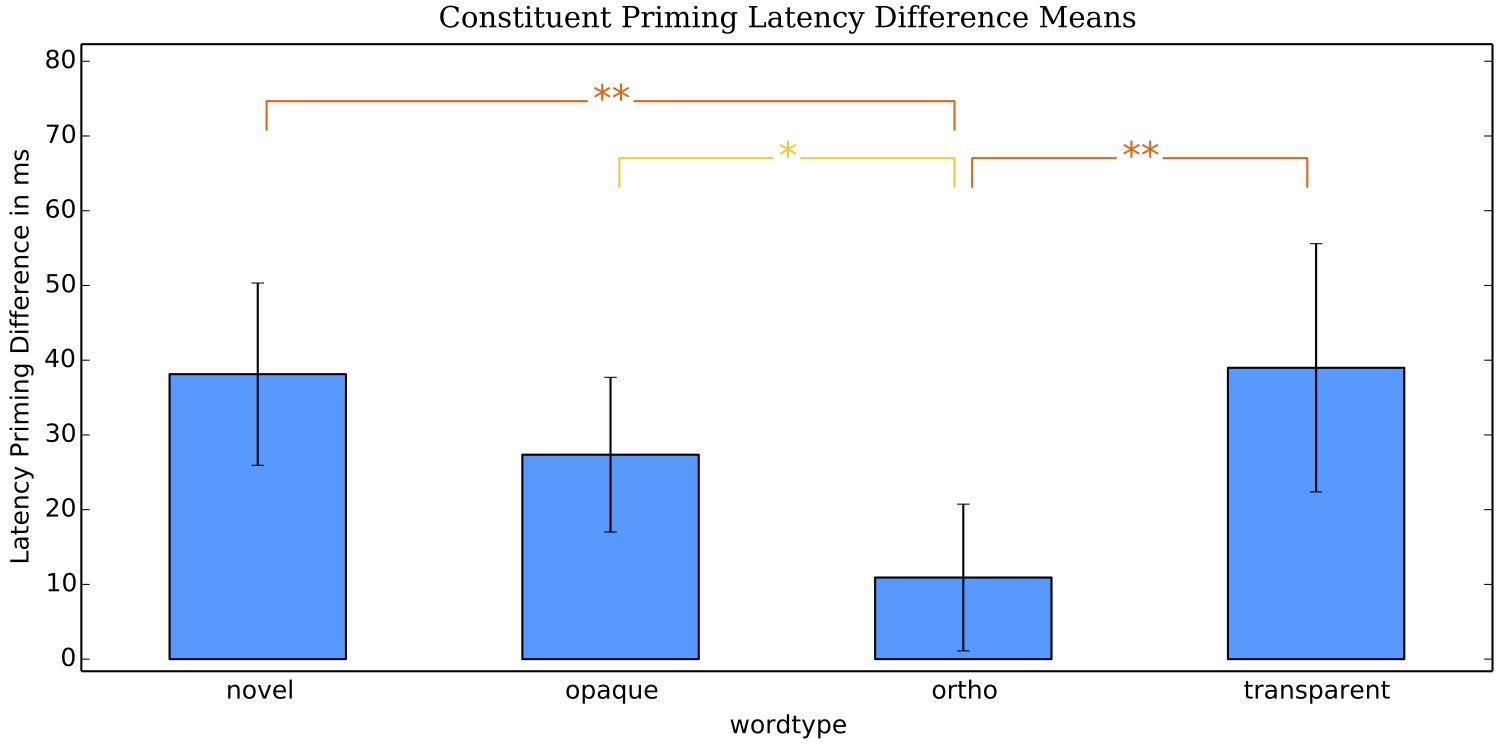
\includegraphics[scale=0.33]{images/latency_constituent_analysis}
\par\end{centering}
\caption{\label{fig:latency} Constituent Priming Differences in Latency Times}
\end{figure}

\begin{figure}
\begin{centering}
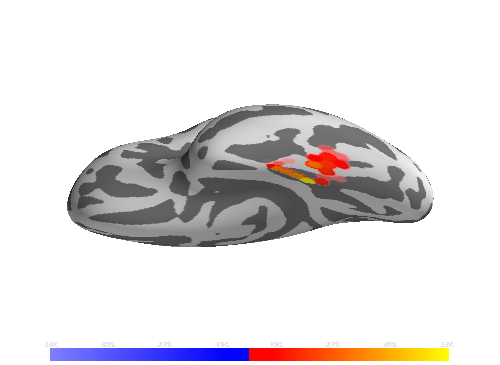
\includegraphics[scale=0.33]{images/target_brain_condition_analysis}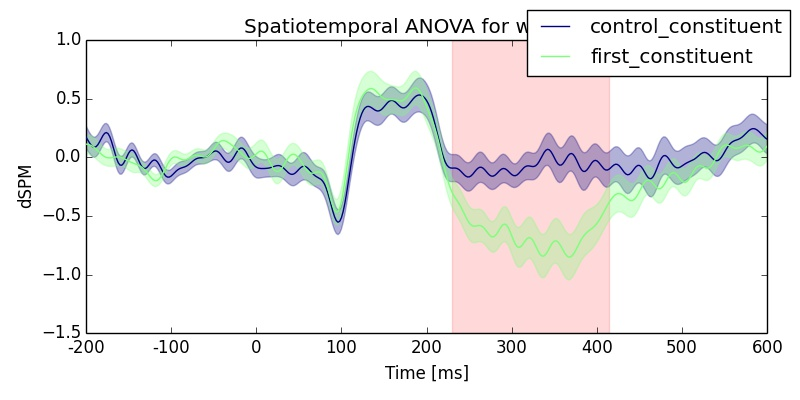
\includegraphics[scale=0.33]{images/target_anova_condition_analysis}
\par\end{centering}
\caption{\label{fig:morph_decomp} Priming Effects in Left Fusiform (VWFA)}
\end{figure}


\begin{figure}
\begin{centering}
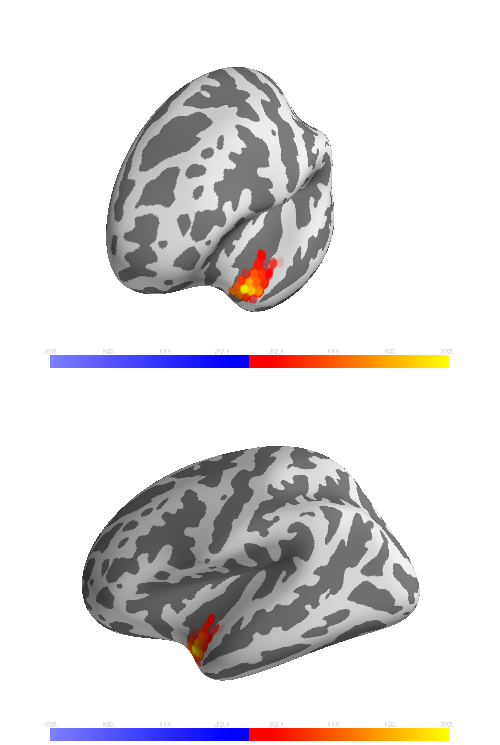
\includegraphics[scale=0.33]{images/opaque_prime_brain_analysis}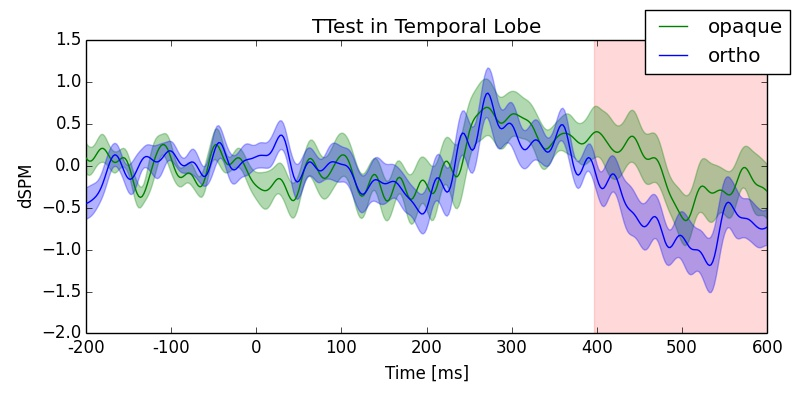
\includegraphics[scale=0.33]{images/opaque_prime_analysis}
\par\end{centering}
\caption{\label{fig:opaque_primes} Opaque vs Ortho Difference in Temporal Lobe}
\end{figure}

\begin{figure}
\begin{centering}
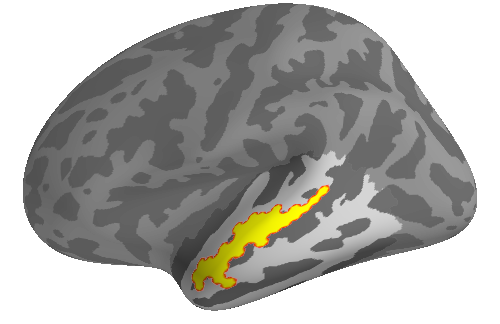
\includegraphics[scale=0.33]{images/transparent_prime_brain_analysis}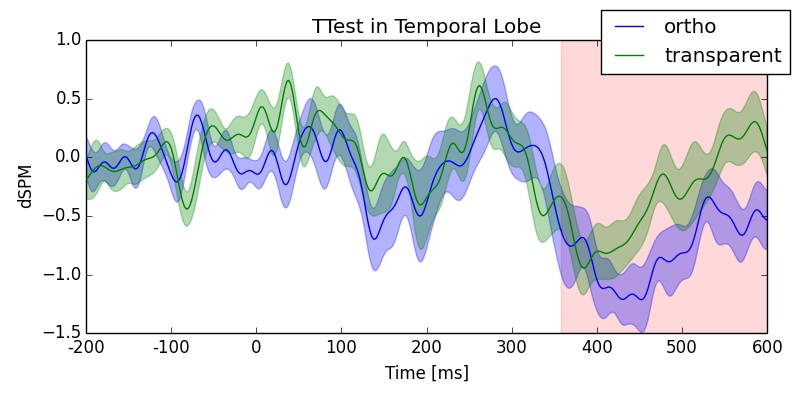
\includegraphics[scale=0.33]{images/transparent_prime_analysis}
\par\end{centering}
\caption{\label{fig:transparent_primes} Transparent vs Ortho Difference in Temporal Lobe}
\end{figure}

\begin{figure}
\begin{centering}
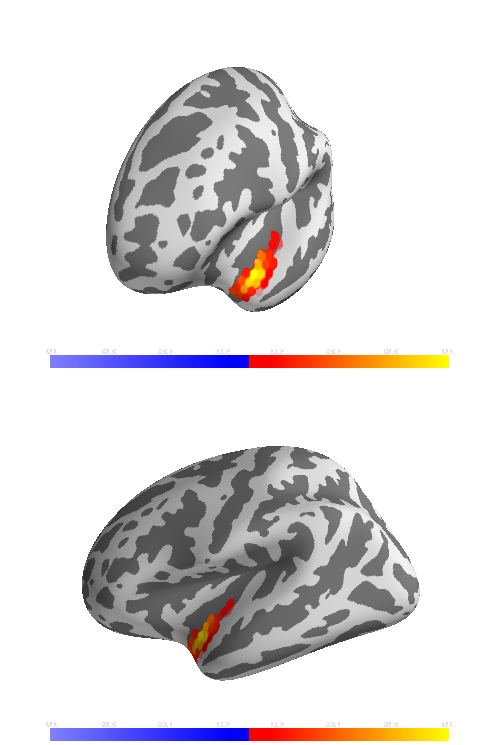
\includegraphics[scale=0.33]{images/novel_prime_brain_analysis}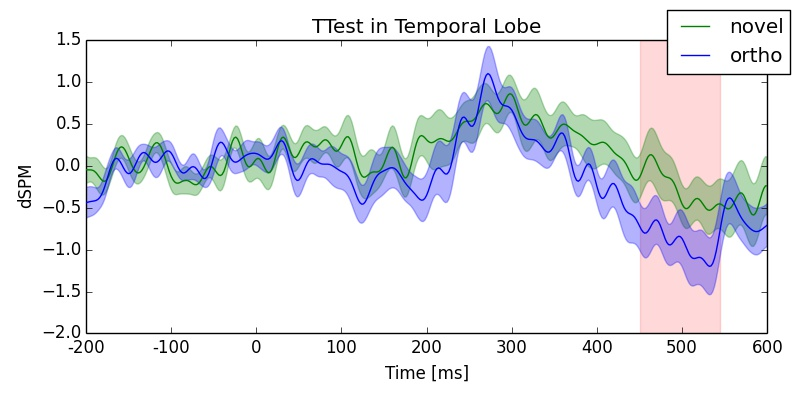
\includegraphics[scale=0.33]{images/novel_prime_analysis}
\par\end{centering}
\caption{\label{fig:novel_primes} Novel vs Ortho Difference in Temporal Lobe}
\end{figure}

\begin{figure}
\begin{centering}
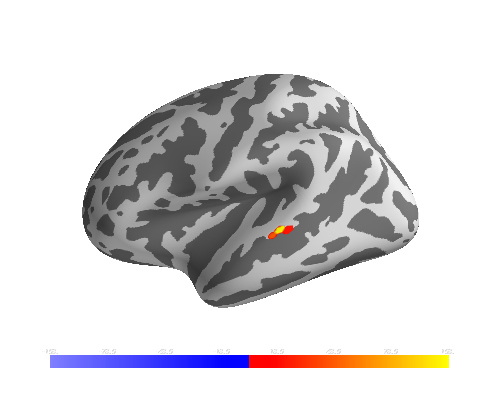
\includegraphics[scale=0.33]{images/target_brain_inter_analysis}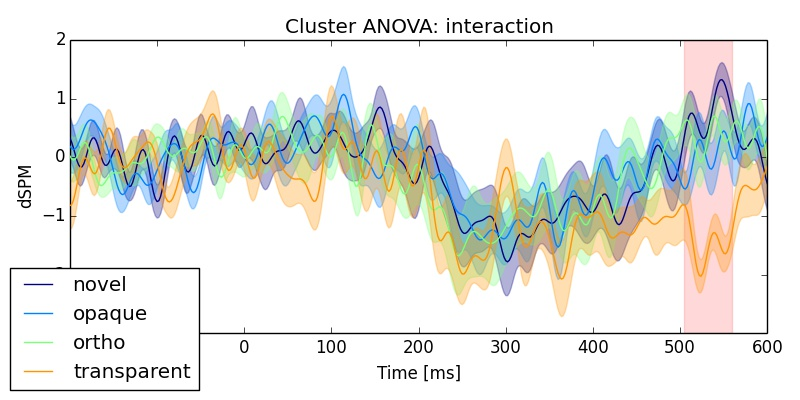
\includegraphics[scale=0.33]{images/target_anova_inter_analysis}
\par\end{centering}
\caption{\label{fig:priming_targets} Constituent Priming Effects in Temporal Lobe}
\end{figure}

\end{document}
